\documentclass{article}
\usepackage{amsmath}
\usepackage{tikz}
\usetikzlibrary{arrows.meta}

\begin{document}

\begin{figure}[h]
    \centering
    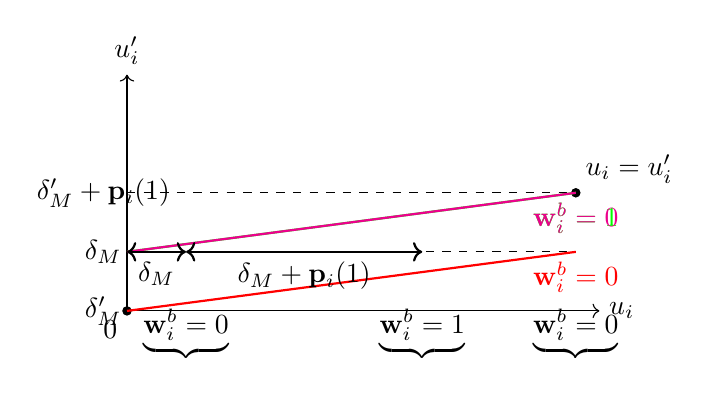
\begin{tikzpicture}[scale=1.5]
        % Axes
        \draw[->] (0,0) -- (4,0) node[right] {$u_i$};
        \draw[->] (0,0) -- (0,2) node[above] {$u'_i$};
        
        % Dashed lines
        \draw[dashed] (0,1) -- (3.8,1);
        \draw[dashed] (0,0.5) -- (3.8,0.5);
        \draw[dashed] (0,0) -- (3.8,0);
        \draw[dashed] (0,0) -- (0,2);
        
        % Points
        \filldraw[black] (0,0) circle (1pt) node[below left] {$0$};
        \filldraw[black] (3.8,1) circle (1pt) node[above right] {$u_i = u'_i$};
        
        % Lines
        \draw[red, thick] (0,0) -- (3.8, 0.5) node[below] {$\mathbf{w}^b_i = 0$};
        \draw[green, thick] (0,0.5) -- (3.8, 1) node[below] {$\mathbf{w}^b_i = 1$};
        \draw[magenta, thick] (0,0.5) -- (3.8, 1) node[below] {$\mathbf{w}^b_i = 0$};
        
        % Labels
        \node at (0.5, -0.2) {$\underbrace{\mathbf{w}^b_i = 0}$};
        \node at (2.5, -0.2) {$\underbrace{\mathbf{w}^b_i = 1}$};
        \node at (3.8, -0.2) {$\underbrace{\mathbf{w}^b_i = 0}$};
        
        % Annotations
        \node at (-0.2, 0.5) {$\delta_M$};
        \node at (-0.2, 1) {$\delta'_M + \mathbf{p}_i(1)$};
        \node at (-0.2, 0) {$\delta'_M$};
        
        % Arrows
        \draw[<->,thick] (0,0.5) -- (0.5,0.5) node[midway,below] {$\delta_M$};
        \draw[<->,thick] (0.5,0.5) -- (2.5,0.5) node[midway,below] {$\delta_M + \mathbf{p}_i(1)$};
    \end{tikzpicture}
    \caption{$u_i$ and $u'_i$ for DISC for $\delta_M + \mathbf{p}_i(1) \geq \delta^{\prime}_M \geq \delta_M$.}
    \label{fig:disc}
\end{figure}

\end{document}